\begin{figure}[htbp]
\centering
\begin{tikzpicture}[x=1cm,y=1cm]
\node[anchor=south west,inner sep=0] at (0,0) {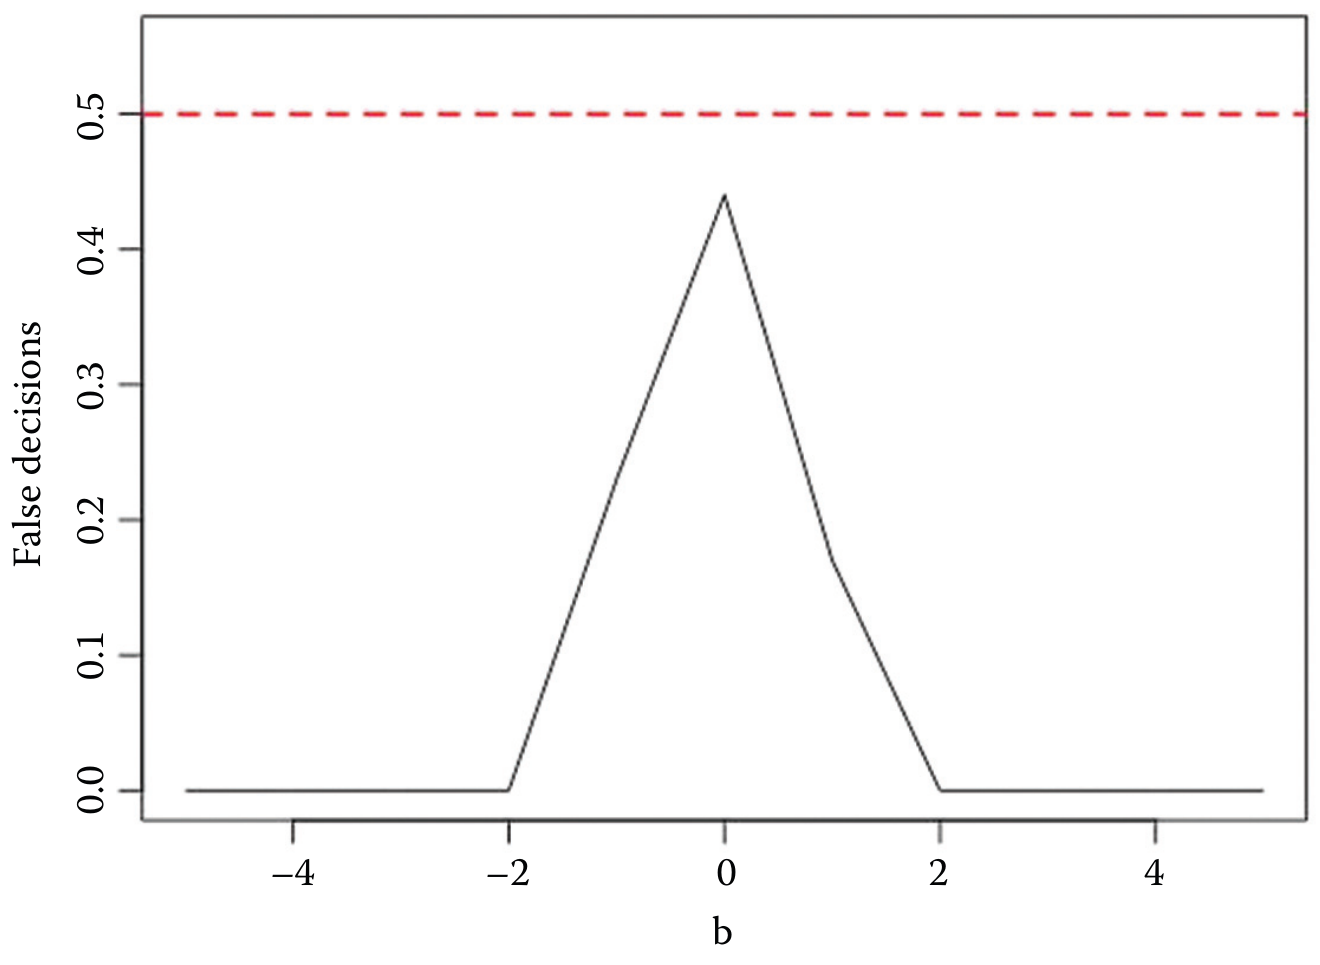
\includegraphics[width=11.5cm]{figures/ch04a_fig23_data.png}};
\fill[white] (0.0585,3.4352) rectangle (0.4569,5.6369);
\node[inner sep=0pt,fill=white,rotate=90,font=\fontsize{8}{8}\selectfont] at (0.2577,4.5360) {误判率};
\end{tikzpicture}
\origfig{23}{假定非线性模型及正态误差分布时，双变量因果发现的误判率。}
\label{fig:ch04a-23}
\end{figure}
